\documentclass[11pt,a4paper]{article}
\usepackage[utf8]{inputenc}
\usepackage[T5]{fontenc}
\usepackage{lmodern}
\usepackage[left=2cm,right=2cm,top=2cm,bottom=2cm]{geometry}
\usepackage{amsmath,amssymb}
\usepackage{booktabs,array}
\usepackage{graphicx}
\usepackage{caption}
\usepackage{enumitem}
\usepackage{microtype}
\graphicspath{{figs/}}
\usepackage[colorlinks=true,linkcolor=blue,citecolor=blue,urlcolor=blue]{hyperref}
\hypersetup{pdftitle={Particle Swarm Optimization: How Individual Memory and Social Information Balance Exploration and Exploitation},pdfauthor={Van Tuan Khai, Huynh Huu Phuc Minh, Le Luong Quoc Trung}}

\captionsetup{labelfont=bf,font=small,labelsep=colon}
\captionsetup[table]{position=above,skip=6pt}
\captionsetup[figure]{position=below,skip=6pt}
\setlist{itemsep=2pt,topsep=3pt,parsep=0pt}
\setlength{\parindent}{0pt}
\setlength{\parskip}{5pt}
\renewcommand{\arraystretch}{1.12}

\newcommand{\pb}{\mathrm{pbest}}
\newcommand{\gb}{\mathrm{gbest}}
\newcommand{\vmax}{v_{\max}}
\newcommand{\Vmax}{V_{\max}}
\newcommand{\tn}[1]{\textit{#1}}

\begin{document}

% ---------------- title ----------------
\begin{center}
{\LARGE\bfseries Particle Swarm Optimization: How Individual Memory and Social Information Balance Exploration and Exploitation\par}
\vspace{4pt}
{\large Seminar S01 Report -- CS420\par}
\vspace{1.4em}
\begin{tabular}{ccc}
Văn Tuấn Khải & Huỳnh Hữu Phúc Minh & Lê Lương Quốc Trung\\[1pt]
{\small 24125032} & {\small 24125068} & {\small 24125084}
\end{tabular}
\end{center}

\begin{abstract}
\noindent Particle Swarm Optimization (PSO) searches a continuous space with a population of particles that are pulled towards their own best positions and towards the best position found by the swarm. This report reviews the original algorithm of Kennedy and Eberhart~\cite{kennedy1995} and the later changes surveyed by Poli et al.~\cite{poli2007}, then studies how PSO balances exploration and exploitation on two 2-D benchmark functions, the unimodal Sphere and the multimodal Rastrigin. We give two worked examples, compare three inertia weights ($\omega=0.4,0.7,0.9$) over five seeds, and compare PSO with Random Search and Hill Climbing under an equal budget of 2,020 function evaluations. With $\omega=0.7$, PSO reached a mean final fitness of $1.0\times10^{-12}$ on Sphere and $1.1\times10^{-6}$ on Rastrigin, and it was the only method to reach a fitness of 0.01 on Rastrigin. The lowest inertia weight gave the best final fitness on both functions, but with a tighter velocity limit one Rastrigin run stalled in a local minimum, so the inertia ranking depends on that limit. A diagnostic run with a strong social pull showed swarm diversity collapsing around a suboptimal basin. These small experiments illustrate rather than establish general behaviour.
\end{abstract}

% ---------------- 1 ----------------
\section{Introduction}
Many practical problems, from tuning a model's hyper-parameters to scheduling, can be written as finding the input that minimises a continuous objective function. When the function has no usable gradient or has many local minima, simple local search methods such as Hill Climbing can stop at the first basin they reach~\cite{nguyen2025}. Population-based methods try to avoid this by searching from many points at once.

PSO is one such method. Each particle remembers the best position it has visited, and the swarm shares the best position found by any particle; every move combines the particle's momentum with random pulls towards these two memories. The method is easy to implement and needs no gradient, which may help explain why it has been applied so widely~\cite[Sect.~6]{poli2007}. Its behaviour, however, depends on how these pulls are weighted.

\textbf{Guiding question.} How does PSO combine individual experience and social information to balance exploration and exploitation? We focus on the role of the personal-best and global-best terms, the effect of the inertia weight, and the risk of premature convergence.

\textbf{Scope and structure.} The scope is deliberately small: two benchmark functions in two dimensions, a global-best PSO with velocity clamping, three inertia-weight settings with five random seeds each, and two baselines with the same evaluation budget. Section~\ref{sec:background} reviews the two source papers, Section~\ref{sec:method} defines the method and works through two numerical examples, Section~\ref{sec:results} presents and discusses the results, and Section~\ref{sec:conclusion} concludes. Findings attributed to the papers are cited; all examples and experiments are our own.

% ---------------- 2 ----------------
\section{Background and Paper Review}\label{sec:background}

\subsection{Origin of PSO and the original algorithm}
PSO came out of simulations of social behaviour rather than from optimisation theory. Kennedy and Eberhart~\cite[pp.~1942--1943]{kennedy1995} started from bird-flocking models and from E.~O. Wilson's~\cite{wilson1975} argument that members of a school of fish profit from the discoveries of the whole school when food is distributed unpredictably; they treated this sharing of information as the core hypothesis behind the method. Because they also wanted to model human social behaviour, which happens in an abstract space where two individuals can hold the same position, their agents were allowed to overlap and behave like points moving through a search space.

An early ``cornfield'' simulation gave each agent two memories: the best position it had found itself (\tn{pbest}) and the best position found by any agent (\tn{gbest}). When the authors removed parts that were not needed, random ``craziness'' and nearest-neighbour velocity matching could be dropped, but \tn{pbest} and \tn{gbest} were both necessary. A pull towards \tn{gbest} much stronger than the pull towards \tn{pbest} made the flock rush prematurely towards local minima, while the reverse made individuals wander; roughly equal pulls worked best~\cite[p.~1945]{kennedy1995}. The final simplified version updates each velocity as
\begin{equation}
\mathbf{v}\leftarrow\mathbf{v}+2\,\mathrm{rand}()\,(\mathbf{pbest}-\mathbf{x})+2\,\mathrm{rand}()\,(\mathbf{gbest}-\mathbf{x}),
\end{equation}
where the factor 2 gives the random multiplier a mean of 1, so that agents overshoot their target about half the time~\cite[p.~1946]{kennedy1995}. A version without the previous velocity was ``quite ineffective at finding global optima''. The reported evidence is small in scale: PSO trained a 13-weight XOR network to the error criterion in an average of 30.7 iterations with 20 agents, trained an Iris classifier as effectively as backpropagation (284 epochs on average), reached 92\% test accuracy on an EEG dataset against 89\% for backpropagation, and found the global optimum of the Schaffer f6 function in every run~\cite[pp.~1945, 1947]{kennedy1995}. The authors called the generalisation result an ``informal indication'', and linked PSO's success to the particles' tendency to overshoot, which balances conservative testing of known regions against exploration of unknown ones~\cite[p.~1947]{kennedy1995}.

\subsection{Parameters and variants}
Poli, Kennedy and Blackwell~\cite{poli2007} published an overview of how the method had changed, which they describe as a snapshot from their own point of view rather than an exhaustive survey. They restate the original algorithm with acceleration coefficients $\varphi_1$ and $\varphi_2$ and note that each velocity component was originally kept within $[-\Vmax,\Vmax]$ (Sect.~2.1 of~\cite{poli2007}). The value $\varphi_1=\varphi_2=2$ used in early work made particle speeds grow without control, and a good $\Vmax$ depended on the problem (Sect.~2.2). Two modifications took over the role of damping. The inertia weight $\omega$ of Shi and Eberhart~\cite{shi1998} multiplies the previous velocity; $1-\omega$ acts like friction, so a high $\omega$ (around 0.9) favours exploration and a low $\omega$ (around 0.4) favours exploitation, and many studies decrease $\omega$ during a run (Sect.~2.3). The constriction coefficient of Clerc and Kennedy~\cite{clerc2002} scales the whole update; a stability analysis of a simplified model showed how to choose it so that a particle converges without $\Vmax$ (Sects.~2.4 and~5.1). Its common setting is algebraically equivalent to an inertia PSO with $\omega=0.7298$ and $c_1=c_2\approx1.49618$ (Sect.~2.4), close to our default $\omega=0.7$ and $c_1=c_2=1.5$.

The review also covers the communication structure of the swarm. In the \tn{gbest} topology every particle is attracted by the best particle of the whole swarm; in the \tn{lbest} ring each particle sees only its neighbours, which converges more slowly but is less vulnerable to local optima, and no topology was best on all functions (Sect.~3.1). Variants include the fully informed particle swarm, swarms with diversity control designed against the ``tendency for the swarm to converge prematurely on local optima'', and velocity-free bare-bones PSO (Sects.~2.5, 4.5, 4.6). Among about 700 application papers, large categories included image analysis, electricity networks and load dispatching, control, scheduling and neural networks (Sect.~6). The authors end with open questions, among them a possible bias towards optima near the centre of the initialisation region (Sect.~7.1), how to treat particles that leave the search space (Sect.~7.2), whether a self-adapting, parameter-free PSO is possible (Sect.~7.4) and how theory could guide the choice of population size, topology and other settings (Sect.~7.5). They conclude that publications on PSO grew exponentially up to 2006 while too few questions had been answered satisfactorily (Sect.~8).

\subsection{Comparison of the two sources}
The 1995 paper introduces a deliberately simple algorithm with fixed coefficients and a handful of demonstrations. The 2007 review shows that later work kept the core idea of pulls towards personal and swarm memories but added explicit control of the dynamics ($\omega$ or $\chi$), studied topology, and collected evidence from a large body of applications. Both identify the same weakness: a swarm that follows its best member too strongly can converge before it finds the global optimum. Our experiments examine this trade-off.

\subsection{PSO and Hill Climbing}
Hill Climbing is a local search method. It keeps a single current state, moves to the best neighbouring state and stops when no neighbour is better. It stores neither the path nor the set of visited states, so it needs very little memory, but it is not systematic and, being greedy, it can get stuck on local optima, ridges or plateaus. Common remedies are limited sideways moves, random choice among the improving moves, taking the first better neighbour, and random restarts~\cite[slides 4--12]{nguyen2025}.

PSO differs in four ways. It keeps a whole population instead of one state. Each particle has a memory (its \tn{pbest}) and the swarm shares information through \tn{gbest} or a neighbourhood. A particle moves by a velocity update that includes momentum and random pulls, so it can pass through worse positions instead of only accepting improvements. Finally, its ``neighbours'' are the particles that influence it through the topology, not adjacent states of the search space. Hill Climbing with random restarts also uses many starting points, but the runs are independent and share no information. The Hill Climbing baseline in our experiments is a stochastic variant for continuous space: it proposes a Gaussian perturbation of the current point and accepts only strict improvements, without restarts (Section~\ref{sec:results}).

\subsection{Critical remarks}
The two papers leave several limits that frame how far our results can be read.
\begin{itemize}
\item \textbf{Small evidence in 1995.} The tests were few, and the authors themselves call the generalisation result an ``informal indication''~\cite[p.~1947]{kennedy1995}.
\item \textbf{Theory is incomplete.} Poli et al.~\cite[Sect.~5]{poli2007} state that no comprehensive mathematical model of PSO exists. The convergence analyses they review assume simplified systems, typically one particle in one dimension without randomness and in stagnation. One of them argues that a particle may converge to a point that is not an optimum, so PSO is not guaranteed to behave as an optimiser (van den Bergh~\cite{vandenbergh2002}, as summarised in~\cite[Sect.~5.1]{poli2007}).
\item \textbf{Parameters interact.} The review notes that parameters cannot be set in isolation (Sect.~2.3) and that rules for population size, run length, initialisation, random-number distributions and topology are still missing (Sect.~7.5). The best topology also depends on the function (Sect.~3.1).
\item \textbf{Premature convergence and slow-down.} The swarm can converge before finding the optimum, or slow down as it approaches an optimum from one side; diversity-control schemes only partly alleviate this (Sects.~4.5 and~7.1).
\item \textbf{Counts are not effectiveness.} The application survey counts papers in one database, so it shows how popular PSO is in each area, not how well it performs there (Sect.~6). This is our reading of the survey, not a claim of its authors.
\end{itemize}

% ---------------- 3 ----------------
\section{Method and Worked Example}\label{sec:method}

\subsection{Problem and objective functions}
We minimise a function $f$ over the box $[-5.12,5.12]^2$. The \textbf{fitness} of a candidate $x$ is its objective value $f(x)$; lower is better. Each call of $f$ on one particle counts as one \textbf{function evaluation}, the cost used to compare algorithms. Two standard benchmarks with $n=2$ are used:
\begin{itemize}
\item \textbf{Sphere:} $f(x)=\sum_i x_i^2$. One basin, minimum $f=0$ at $(0,0)$; it tests convergence speed on a smooth landscape.
\item \textbf{Rastrigin:} $f(x)=10n+\sum_i\bigl(x_i^2-10\cos 2\pi x_i\bigr)$. Same global minimum, but the cosine term creates a grid of local minima near integer coordinates; it tests whether the swarm gets trapped. Because it is computed as a difference of two numbers close to 20, values below about $10^{-13}$ are at floating-point resolution and are treated as the global minimum.
\end{itemize}

\subsection{Algorithm}\label{sec:algorithm}
We use the global-best PSO with an inertia weight in the form of Poli et al.~\cite[Eq.~2]{poli2007}. For particle $i$ at iteration $t$:
\begin{align}
v_i(t+1) &= \omega\, v_i(t) + c_1 r_1\otimes\bigl(\pb_i-x_i(t)\bigr) + c_2 r_2\otimes\bigl(\gb-x_i(t)\bigr),\label{eq:v}\\
x_i(t+1) &= x_i(t)+v_i(t+1).\label{eq:x}
\end{align}
The three terms are inertia (keeps part of the previous motion), the cognitive term (pull towards the particle's own best) and the social term (pull towards the swarm's best). The assignment sheet writes the position update with $v(t)$; we use the newly computed velocity $v(t+1)$, which is the form in Poli et al.~\cite{poli2007}. Table~\ref{tab:symbols} defines every symbol.

\begin{table}[ht]
\centering
\caption{Symbols and values used in this work.}\label{tab:symbols}
\small
\begin{tabular}{@{}p{2.0cm}p{9.0cm}p{5.0cm}@{}}
\toprule
\textbf{Symbol} & \textbf{Meaning} & \textbf{Range or value used}\\
\midrule
$x_i(t)$ & Position of particle $i$, a candidate solution & $[-5.12,5.12]^2$\\
$v_i(t)$ & Velocity of particle $i$ (step taken in one iteration) & each component in $[-10.24,10.24]$\\
$\pb_i$ & Best position found so far by particle $i$ & updated when $f$ improves\\
$\gb$ & Best position found so far by the whole swarm & updated every iteration\\
$\omega$ & Inertia weight: share of the previous velocity kept & 0.4, 0.7 (default), 0.9\\
$c_1,c_2$ & Cognitive and social acceleration coefficients & 1.5 and 1.5\\
$r_1,r_2$ & Uniform random numbers, new for every particle, dimension and iteration & $U(0,1)$\\
$\otimes$ & Component-wise multiplication & \\
$N,T$ & Number of particles, number of iterations & 20 and 100 (5 and 5 in Section~\ref{sec:five})\\
$\vmax$ & Velocity limit & 10.24 (domain width)\\
\bottomrule
\end{tabular}
\end{table}

The algorithm proceeds as follows:
\begin{enumerate}
\item Place $N$ particles uniformly at random in the domain and draw velocities uniformly from $[-\vmax,\vmax]$.
\item Evaluate $f$ for every particle; set $\pb_i=x_i$ and $\gb$ to the best $\pb$.
\item For $t=1,\dots,T$: draw $r_1$ and $r_2$; update every velocity and clip it to $[-\vmax,\vmax]$; move every particle and clip it to the domain; evaluate $f$; replace $\pb_i$ when $f$ improves; then update $\gb$.
\item Return $\gb$ and $f(\gb)$.
\end{enumerate}

Velocity clamping follows the original PSO~\cite[Sect.~2.2]{poli2007}; positions outside the domain are moved to the nearest boundary. We set $\vmax=10.24$, the domain width, following the rule $V_{\max}=X_{\max}$ that Poli et al.~\cite[Sects.~2.3--2.4]{poli2007} describe for PSOs with an inertia weight or constriction. A tighter limit ($\vmax=2.0$, about 20\% of the width) was used in an earlier version of our experiments; Section~\ref{sec:inertia} reports how it changes the results. All particles in one iteration use the \tn{gbest} of the previous iteration. With $N=20$ and $T=100$, one run uses $20+20\times100=\mathbf{2{,}020}$ function evaluations.

\subsection{Worked example 1: one update step in one dimension}
We take $f(x)=x^2$, $\omega=0.7$, $c_1=c_2=1.5$, two particles and fixed random numbers, with no velocity limit. At iteration 0 each \tn{pbest} equals the particle's own position, and $\gb=-2$ because $f(-2)=4<f(3)=9$.

\begin{table}[ht]
\centering
\caption{One update step for two particles on $f(x)=x^2$.}\label{tab:step}
\footnotesize
\setlength{\tabcolsep}{3pt}
\begin{tabular}{@{}cccccrcp{3.4cm}rrr@{}}
\toprule
\textbf{Particle} & $x(0)$ & $v(0)$ & $r_1$ & $r_2$ & Inertia $\omega v$ & Cogn. & Social $c_2r_2(\gb-x)$ & $v(1)$ & $x(1)$ & $f(x(1))$\\
\midrule
1 & 3 & 0.5 & 0.4 & 0.6 & 0.35 & 0 & $1.5\times0.6\times(-5)=-4.5$ & $-4.15$ & $-1.15$ & 1.3225\\
2 & $-2$ & $-0.5$ & 0.8 & 0.3 & $-0.35$ & 0 & 0 & $-0.35$ & $-2.35$ & 5.5225\\
\bottomrule
\end{tabular}
\end{table}

The cognitive term is zero for both particles because $\pb=x$ at iteration 0. Particle 2 is the current \tn{gbest}, so its social term is also zero and inertia alone moves it further from the optimum ($f$ rises from 4 to 5.5225). Particle 1 is pulled strongly towards particle 2, overshoots the optimum and lands at $-1.15$; its fitness falls from 9 to 1.3225, so $\pb_1=-1.15$ and the new $\gb=-1.15$. One particle can get worse while the swarm's best improves.

\subsection{Worked example 2: five particles over five iterations}\label{sec:five}
We ran the full algorithm on the 2-D Sphere function with $N=5$, $T=5$, seed 42 and the default parameters. Table~\ref{tab:states} gives every particle's state at iterations 0 and 1.

\begin{table}[ht]
\centering
\caption{Particle states at iterations 0 and 1 (Sphere, seed 42). At iteration 0, $\pb_i=x_i$; at iteration 1, only particles 3 and 5 improved, so only their $\pb_i$ changed. Positions are clipped to the domain $[-5.12,5.12]^2$.}\label{tab:states}
\footnotesize
\setlength{\tabcolsep}{3pt}
\begin{tabular}{@{}lrrrrrrrrrr@{}}
\toprule
\textbf{Particle} & $x_1(0)$ & $x_2(0)$ & $v_1(0)$ & $v_2(0)$ & $f(0)$ & $x_1(1)$ & $x_2(1)$ & $v_1(1)$ & $v_2(1)$ & $f(1)$\\
\midrule
1 & 2.8053 & $-0.6259$ & $-2.6461$ & 8.7401 & 8.2615 & 0.9531 & 5.1200 & $-1.8522$ & 6.1181 & 27.1227\\
2 & 3.6720 & 2.0210 & 2.9464 & 6.6102 & 17.5685 & 5.1200 & 5.1200 & 1.6388 & 3.1562 & 52.4288\\
3 & $-4.1556$ & 4.8704 & $-1.1589$ & $-5.5862$ & 40.9897 & $-0.0640$ & $-0.6020$ & 4.0916 & $-5.4724$ & 0.3665\\
4 & 2.6741 & 2.9293 & 1.1179 & $-8.9330$ & 15.7314 & 3.4822 & $-5.1200$ & 0.8081 & $-8.7899$ & 38.3399\\
5 & $-3.8081$ & $-0.5080$ & 6.7099 & 2.6965 & 14.7599 & 3.1398 & 1.2611 & 6.9479 & 1.7691 & 11.4486\\
\midrule
gbest & 2.8053 & $-0.6259$ & & & 8.2615 & $-0.0640$ & $-0.6020$ & & & 0.3665\\
\bottomrule
\end{tabular}
\end{table}

\textbf{Particle 2, step by step.} The random numbers used were $r_1=(0.9707,0.8931)$ and $r_2=(0.3258,0.3705)$. In dimension 1, the inertia term is $0.7\times2.9464=2.0625$, the cognitive term is 0 and the social term is $1.5\times0.3258\times(2.8053-3.6720)=-0.4236$, so $v_1(1)=1.6388$ and $x_1=3.6720+1.6388=5.3108$, which is moved to the boundary 5.12. In dimension 2, inertia gives $0.7\times6.6102=4.6271$ and the social term is $1.5\times0.3705\times(-0.6259-2.0210)=-1.4709$, so $v_2(1)=3.1562$ and $x_2=5.1772$, again moved to 5.12; the new fitness is $f=52.4288$, worse than before. No velocity reached the limit, but particles 1, 2 and 4 were moved to the boundary in at least one coordinate at iteration 1, because the initial velocities are drawn from $[-10.24,10.24]$. Over five iterations $f(\gb)$ fell from 8.2615 to 0.3665 at iteration 1 (particle 3) and did not improve afterwards (Figure~\ref{fig:swarm}).

\begin{figure}[ht]
\centering
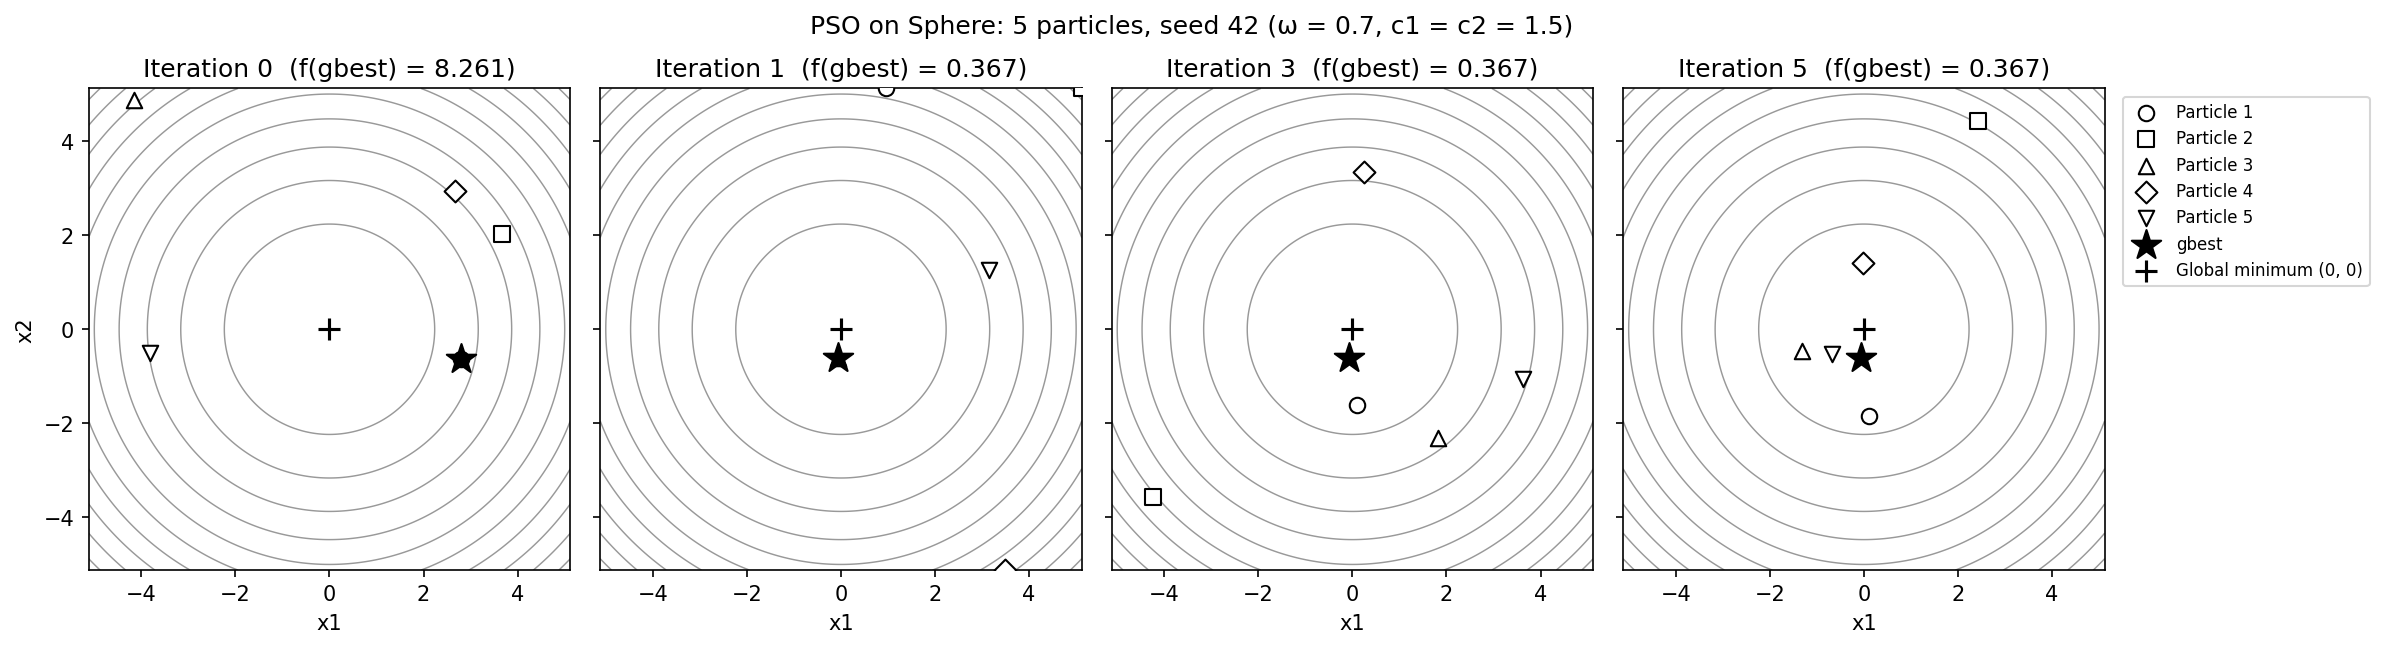
\includegraphics[width=0.95\linewidth]{fig_swarm_sphere.png}
\caption{Five particles on the Sphere contours at iterations 0, 1, 3 and 5 (seed 42). The star marks \tn{gbest} and the cross the global minimum. Source: team experiment.}\label{fig:swarm}
\end{figure}

\subsection{Experimental setup}
To study the inertia weight we compare \textbf{A} ($\omega=0.4$), \textbf{B} ($\omega=0.7$) and \textbf{C} ($\omega=0.9$), all with $c_1=c_2=1.5$, $N=20$ and $T=100$, on both functions with seeds 0 to 4. For the comparison with local search, Random Search samples uniformly from the domain, and Hill Climbing starts from one uniform point, adds Gaussian noise with $\sigma=0.3$ per coordinate, clips to the domain and accepts only strict improvements, without restarts. Both baselines receive exactly 2,020 evaluations per run, counting initialisation and rejected proposals, and use the same seeds. We report the final best fitness (mean, sample standard deviation, best and worst over five seeds) and the number of evaluations until the best fitness first falls below 0.01. Each run is fully determined by its seed; the code and raw results are in the team's notebooks.

% ---------------- 4 ----------------
\section{Results and Discussion}\label{sec:results}

\subsection{Equal-budget comparison}
\begin{table}[ht]
\centering
\caption{Final best fitness after 2,020 evaluations (five seeds; lower is better).}\label{tab:final}
\small
\begin{tabular}{@{}llrrrr@{}}
\toprule
\textbf{Function} & \textbf{Method} & \textbf{Mean} & \textbf{SD} & \textbf{Best} & \textbf{Worst}\\
\midrule
Sphere & PSO ($\omega=0.7$) & 1.004e$-$12 & 1.250e$-$12 & 1.502e$-$15 & 2.433e$-$12\\
Sphere & Random Search & 1.397e$-$02 & 1.605e$-$02 & 1.216e$-$03 & 4.154e$-$02\\
Sphere & Hill Climbing & 2.602e$-$04 & 2.883e$-$04 & 4.341e$-$05 & 6.466e$-$04\\
Rastrigin & PSO ($\omega=0.7$) & 1.070e$-$06 & 2.345e$-$06 & 1.595e$-$11 & 5.264e$-$06\\
Rastrigin & Random Search & 1.232e+00 & 8.268e$-$01 & 2.408e$-$01 & 2.484e+00\\
Rastrigin & Hill Climbing & 5.205e+00 & 4.557e+00 & 1.991e+00 & 1.304e+01\\
\bottomrule
\end{tabular}
\end{table}

\begin{table}[ht]
\centering
\caption{Evaluations until the best fitness first falls below 0.01 (mean over the seeds that reached it). PSO is recorded at the end of each 20-evaluation batch.}\label{tab:hits}
\small
\begin{tabular}{@{}llrr@{}}
\toprule
\textbf{Function} & \textbf{Method} & \textbf{Mean evaluations} & \textbf{Seeds reaching 0.01}\\
\midrule
Sphere & PSO ($\omega=0.7$) & 216.0 & 5/5\\
Sphere & Random Search & 659.0 & 3/5\\
Sphere & Hill Climbing & 42.6 & 5/5\\
Rastrigin & PSO ($\omega=0.7$) & 1004.0 & 5/5\\
Rastrigin & Random Search & not reached & 0/5\\
Rastrigin & Hill Climbing & not reached & 0/5\\
\bottomrule
\end{tabular}
\end{table}

On Sphere, Hill Climbing reached 0.01 in all five runs after a mean of 42.6 evaluations, compared with 216.0 for PSO (Table~\ref{tab:hits}). Its progress then slowed, while PSO kept improving (Figure~\ref{fig:compare}) and finished with a mean of $1.004\times10^{-12}$, against $2.602\times10^{-4}$ for Hill Climbing and $1.397\times10^{-2}$ for Random Search (Table~\ref{tab:final}). A single local search gave rapid initial progress on the smooth objective; PSO was stronger when the goal was final accuracy under this budget.

On Rastrigin, PSO reached 0.01 in all five runs after 1,004 evaluations on average, and neither baseline reached it. Random Search finished ahead of Hill Climbing (means 1.232 and 5.205), while PSO averaged $1.070\times10^{-6}$. Uniform sampling kept trying points in different basins, whereas the single-start Hill Climbing, which accepts only improvements with a fixed step scale, rarely left the basin it reached first. The comparison measures fitness against evaluations; runtime was outside the scope of the experiment.

\begin{figure}[ht]
\centering
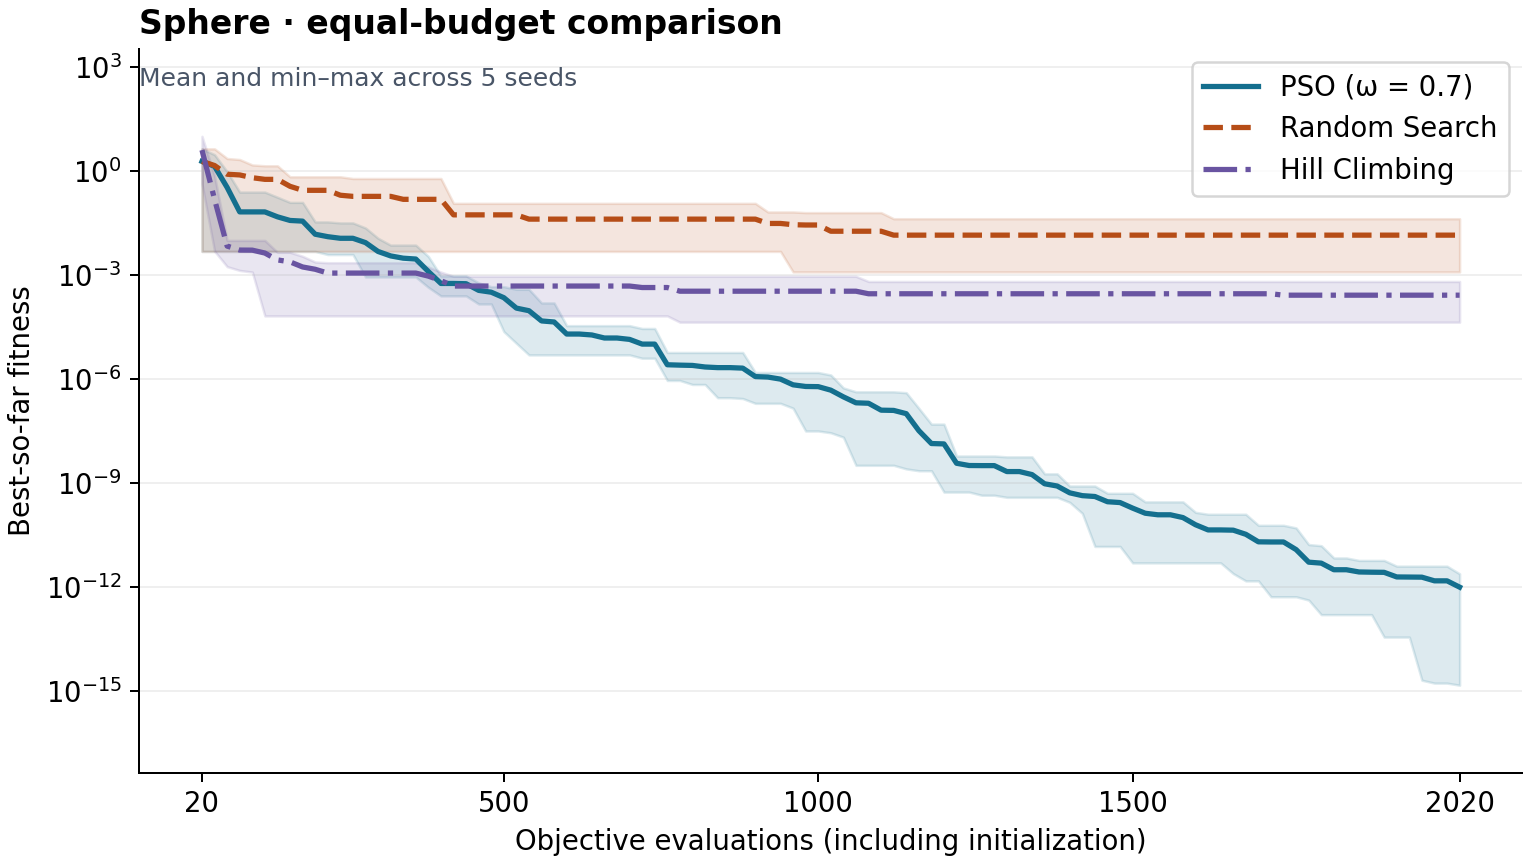
\includegraphics[width=0.49\linewidth]{fig_compare_sphere.png}\hfill
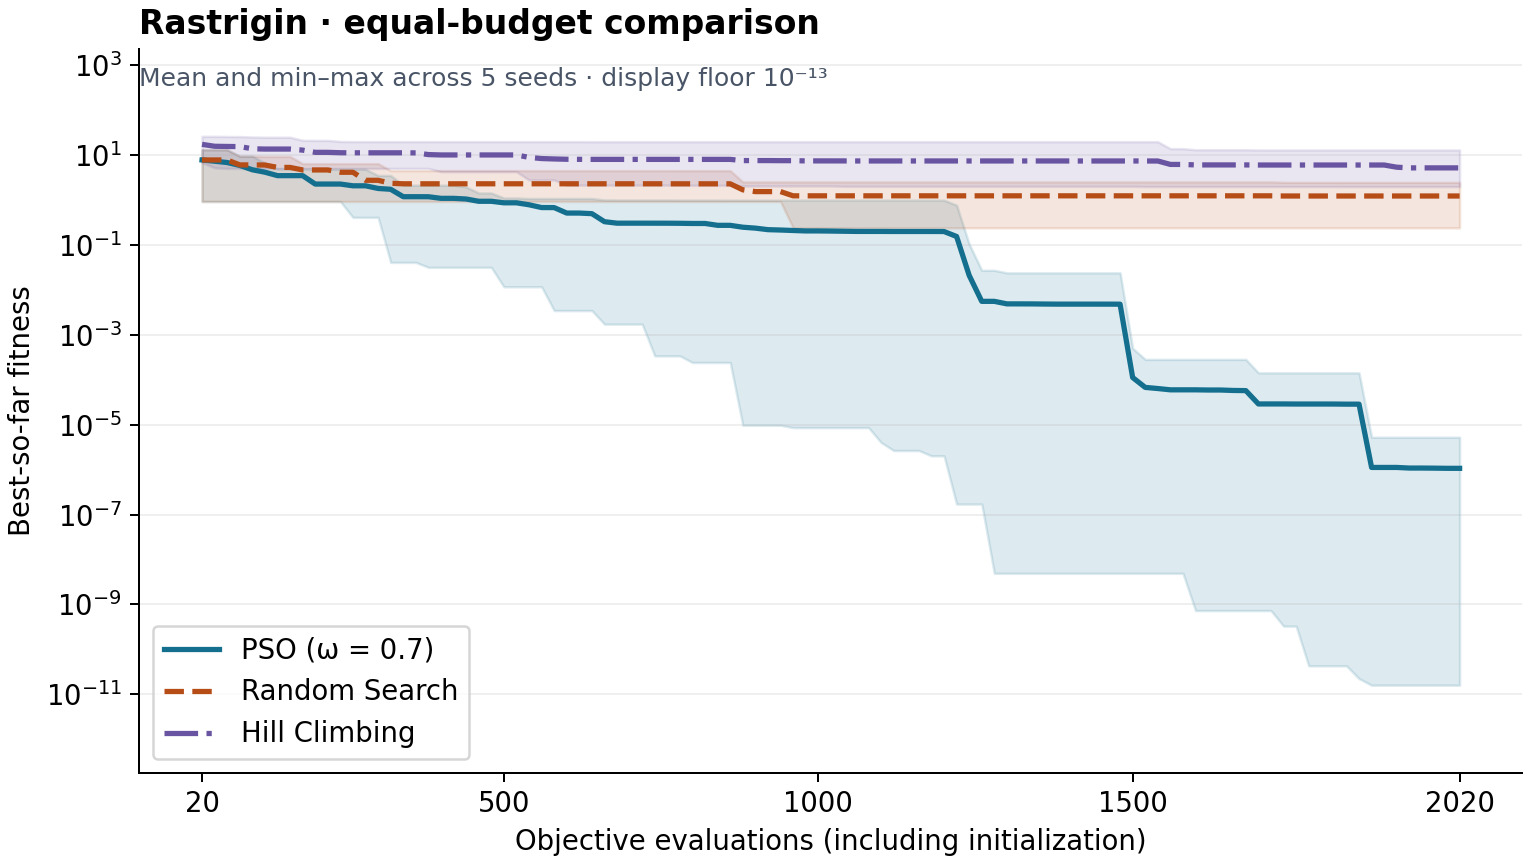
\includegraphics[width=0.49\linewidth]{fig_compare_rastrigin.png}
\caption{Best-so-far fitness against function evaluations on Sphere (left) and Rastrigin (right): mean and min--max range over five seeds. The Rastrigin plot uses a display floor of $10^{-13}$. For PSO, 20 evaluations correspond to one iteration (iteration $k$ at $20\times(k+1)$ evaluations, so 2,020 evaluations is iteration 100); Random Search and Hill Climbing have no iterations, so evaluations are the common axis. Source: team experiments.}\label{fig:compare}
\end{figure}

\subsection{Sensitivity to the inertia weight}\label{sec:inertia}
\begin{table}[ht]
\centering
\caption{Mean final PSO fitness for three inertia weights (five seeds, 2,020 evaluations, $c_1=c_2=1.5$, $\vmax=10.24$).}\label{tab:omega}
\small
\begin{tabular}{@{}lrrr@{}}
\toprule
\textbf{Function} & \textbf{A ($\omega=0.4$)} & \textbf{B ($\omega=0.7$)} & \textbf{C ($\omega=0.9$)}\\
\midrule
Sphere & 8.813e$-$30 & 1.004e$-$12 & 3.598e$-$04\\
Rastrigin & 0 & 1.070e$-$06 & 1.644e$-$01\\
\bottomrule
\end{tabular}
\end{table}

The lowest inertia gave the best final mean on both functions, and the ranking A $<$ B $<$ C held on Sphere and on Rastrigin (Table~\ref{tab:omega}). On Sphere there is only one basin, so strong damping lets the swarm settle and refine quickly; with $\omega=0.9$ the swarm was still converging when the budget ran out (mean $3.6\times10^{-4}$). On Rastrigin, all five runs with $\omega=0.4$ reached the global minimum (values at floating-point resolution), $\omega=0.7$ averaged $1.1\times10^{-6}$, and $\omega=0.9$ ended at a mean of 0.164, dominated by one run at 0.67 (the other four were below 0.07). This matches the interpretation of $1-\omega$ as friction in Poli et al.~\cite{poli2007}: low $\omega$ slows the particles and favours exploitation, which paid off on both landscapes within 100 iterations, whereas $\omega=0.9$ kept them moving too much for this budget. Only $\omega$ was varied, so the sweep shows sensitivity to $\omega$ under these settings; ranking the effects of $c_1$ and $c_2$ would need a separate controlled sweep.

Our velocity limit $\vmax=10.24$ equals the domain width, the rule $V_{\max}=X_{\max}$ discussed in~\cite[Sects.~2.3--2.4]{poli2007}. An earlier version of our experiments used the tighter limit $\vmax=2.0$, about 20\% of the domain width, so we repeated the sweep with $\vmax=2.0$, 5.12 and with no clamp (Table~\ref{tab:vmax}; with no clamp, initial velocities are still drawn from $\pm10.24$). On Sphere the ranking A $<$ B $<$ C held for every limit. On Rastrigin, $\omega=0.7$ ended near zero in every setting (mean at most $1.1\times10^{-6}$), but with $\vmax\le5.12$ one of the five $\omega=0.4$ runs stalled near 0.995, which made $\omega=0.7$ the best setting there; with $\vmax=10.24$ or no clamp all five $\omega=0.4$ runs reached the global minimum. The ranking of $\omega$ on Rastrigin therefore depends on the velocity limit.

\begin{table}[ht]
\centering
\caption{Mean final PSO fitness by velocity limit (five seeds, 2,020 evaluations, $c_1=c_2=1.5$). The default is $\vmax=10.24$; ``none'' means no clamp.}\label{tab:vmax}
\small
\begin{tabular}{@{}lcrrrr@{}}
\toprule
\textbf{Function} & $\omega$ & $\vmax=2.0$ & $5.12$ & $10.24$ (default) & none\\
\midrule
Sphere & 0.4 & 5.455e$-$31 & 2.917e$-$30 & 8.813e$-$30 & 8.813e$-$30\\
Sphere & 0.7 & 1.795e$-$13 & 5.781e$-$13 & 1.004e$-$12 & 1.265e$-$12\\
Sphere & 0.9 & 4.158e$-$05 & 1.151e$-$04 & 3.598e$-$04 & 3.270e$-$04\\
Rastrigin & 0.4 & 1.990e$-$01 & 1.990e$-$01 & 0 & 0\\
Rastrigin & 0.7 & 2.077e$-$07 & 1.963e$-$08 & 1.070e$-$06 & 9.626e$-$09\\
Rastrigin & 0.9 & 8.452e$-$03 & 4.430e$-$02 & 1.644e$-$01 & 6.735e$-$02\\
\bottomrule
\end{tabular}
\end{table}

\subsection{Premature convergence}
In a separate Rastrigin diagnostic we ran five particles with $\omega=0.4$, $c_1=0.5$ and $c_2=2.5$ for 100 iterations over seeds 0 to 19. All 20 runs finished above 0.9 (the smallest final fitness was 0.995). Seed 0, the first, ended at a verified local minimum near $(0,\,-0.994959)$ with fitness 0.994959, while the global value is 0. The mean distance of the particles to the swarm centroid fell from 4.184 to $3.01\times10^{-9}$, so the swarm had collapsed onto one point. The default run with the same seed kept a final mean distance of 0.0552 and found a point with fitness $1.570\times10^{-8}$ (Figure~\ref{fig:trap}).

A strong pull towards \tn{gbest} and a small population are plausible contributors to this rapid loss of diversity. This mirrors the 1995 observation that a relatively high \texttt{g\_increment} makes the flock rush prematurely towards local minima. Low inertia alone is not enough: in the inertia sweep (Table~\ref{tab:omega}), $\omega=0.4$ with the default $c_1=c_2=1.5$ and 20 particles reached the global minimum in all five runs. The diagnostic changes several settings at once ($\omega$, $c_1$, $c_2$ and the number of particles) and uses 505 evaluations against 2,020 for the default run, so it shows how a swarm can converge tightly around a suboptimal basin without measuring how much each parameter contributed.

\begin{figure}[ht]
\centering
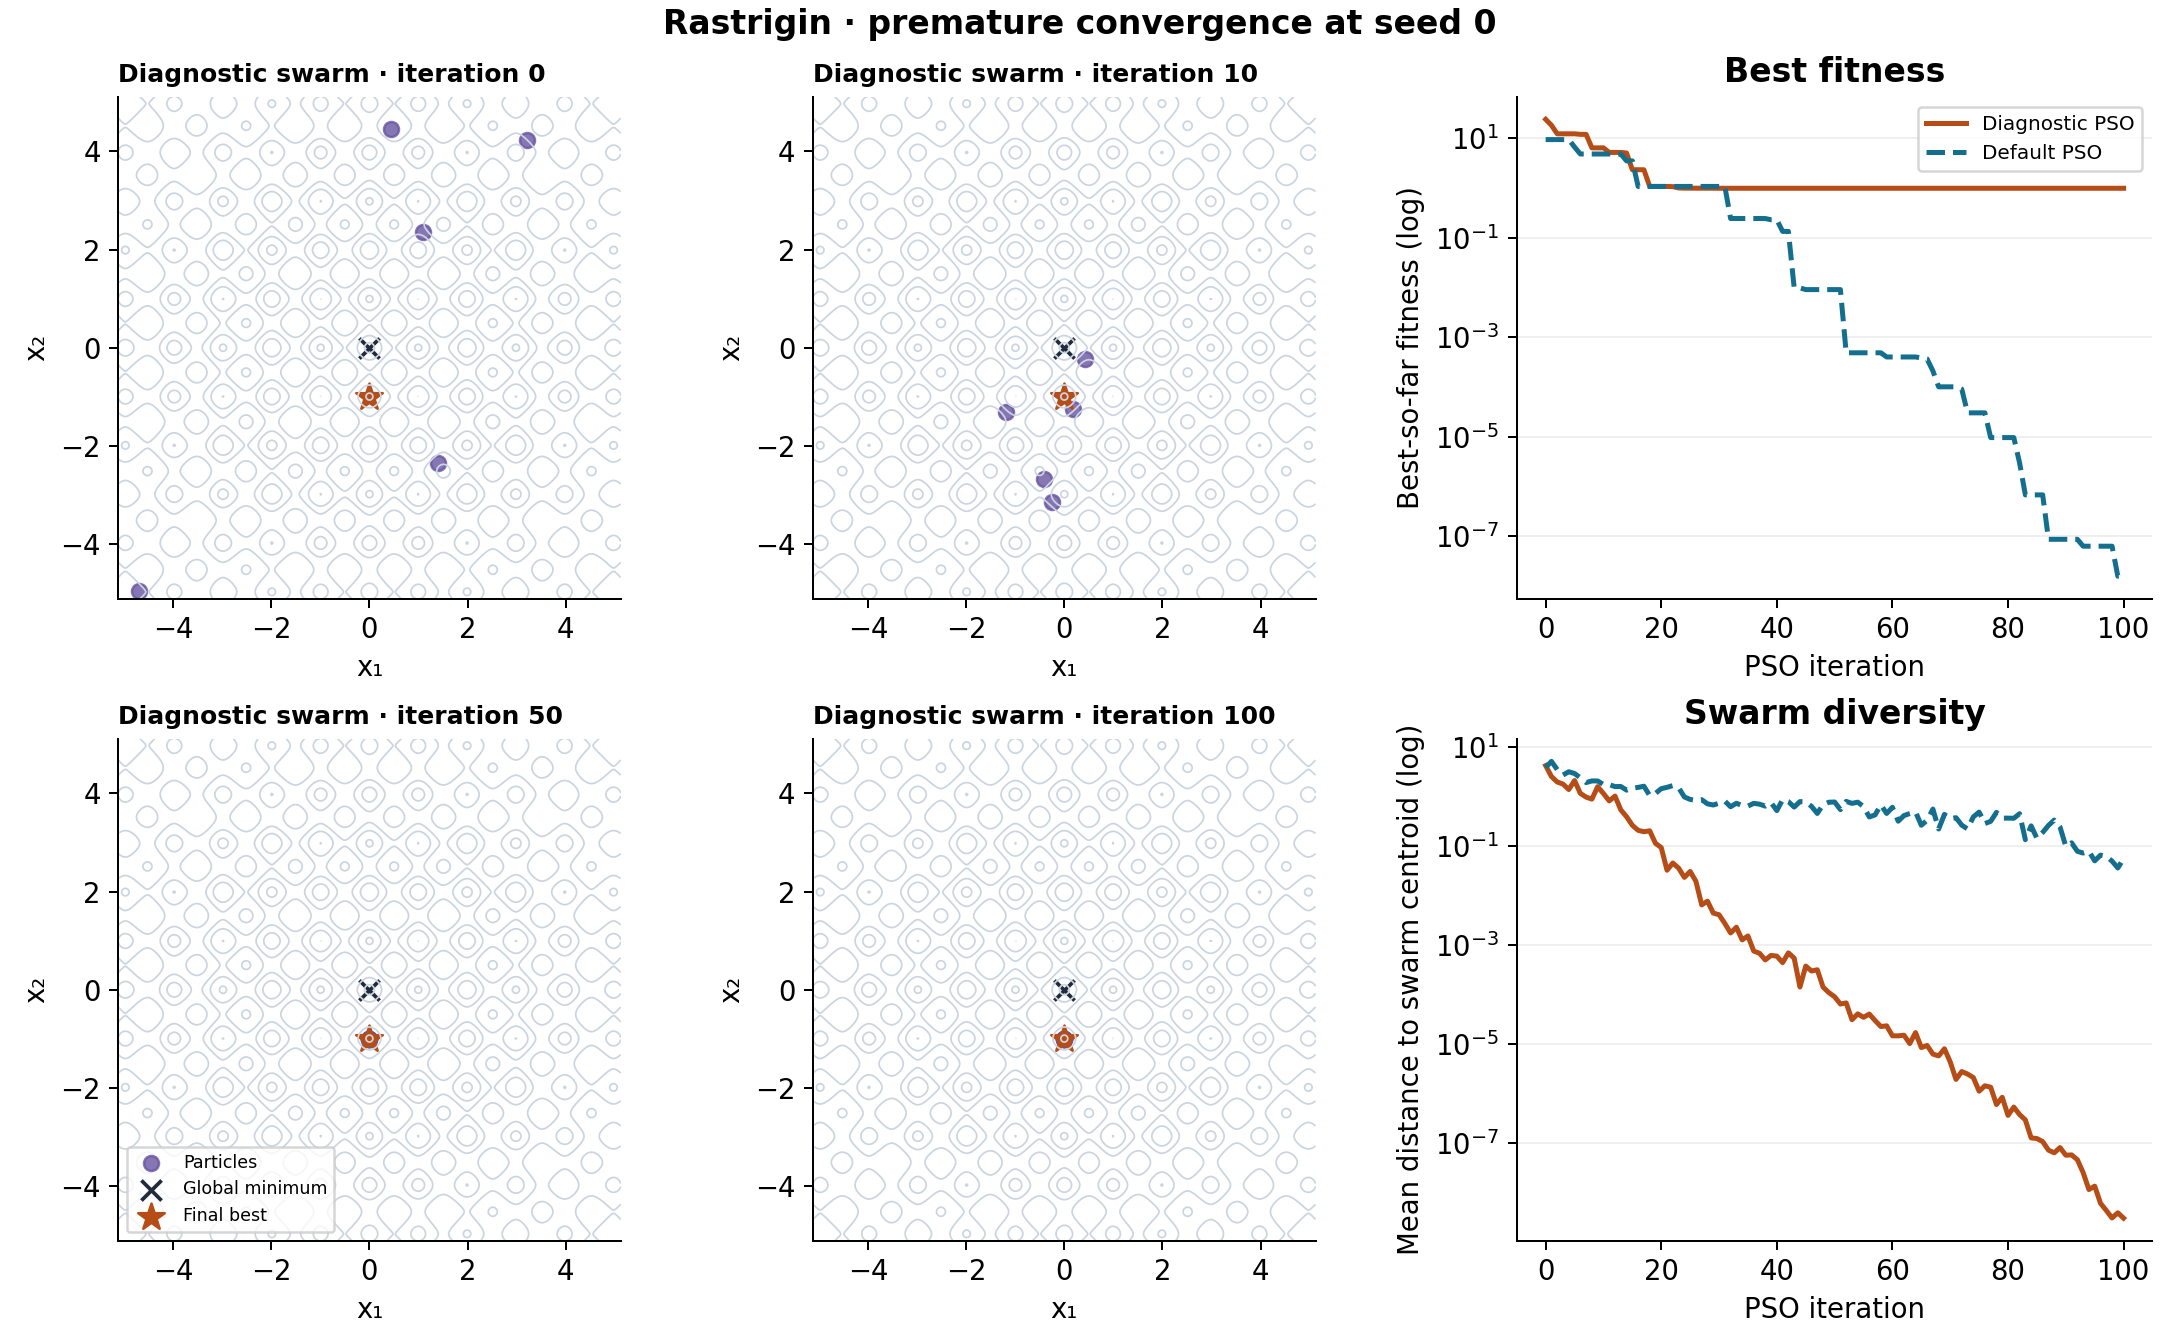
\includegraphics[width=0.82\linewidth]{fig_local_optimum.png}
\caption{Premature convergence on Rastrigin (seed 0): diagnostic swarm at iterations 0, 10, 50 and 100, with best fitness and swarm diversity for the diagnostic and default runs. Source: team experiment.}\label{fig:trap}
\end{figure}

\subsection{Applications and strengths}
\textbf{Range of applications.} Poli et al.~\cite[Sect.~6]{poli2007} counted more than 1,100 PSO publications in IEEE Xplore, about 700 of them applications, and grouped them into 26 categories. The largest were image and video analysis (51 papers), electricity networks and load dispatching (48) and control (47), followed by electronics and electromagnetics, antenna design, power generation, scheduling, communication networks, clustering and classification, and neural networks. The authors found PSO most promising for multimodal problems and for problems where no specialised method exists or where specialised methods give unsatisfactory results. These counts show how often PSO was used by 2007, not how well it performs in each field. We describe two applications in which the objective has several local optima, as in our Rastrigin experiment.

\textbf{Application 1: photovoltaic maximum power point tracking.} Alshareef et al.~\cite{alshareef2019} used a PSO-based method to track the maximum power point of a photovoltaic array under partial shading, where the power curve has several local peaks. Each particle is a converter duty cycle and its fitness is the measured output power. In hardware tests with three particles and three shading scenarios, standard PSO ($\omega=0.4$) reached 94--99\% efficiency, while perturb-and-observe, a local method, was trapped on a local peak in two scenarios (35.87\,W against 40.76\,W rated in the first, 44.1\,W against 76.53\,W in the third). Their proposed variant, which applies perturb-and-observe to the best particle, converged faster (1.9--2.4\,s against 3.0--4.6\,s). This resembles our Hill Climbing baseline on Rastrigin, although their problem has one variable and ours has two.

\textbf{Application 2: UAV path planning.} Phung and Ha~\cite{phung2021} used a PSO variant, spherical vector-based PSO (SPSO), to plan the flight path of an unmanned aerial vehicle among several threats. The cost to be minimised is a weighted sum of four terms: path length, threat, smoothness and flight height. In classic PSO a particle is a list of 3D waypoints. In SPSO it is a list of vectors, each with a length, an elevation angle and an azimuth angle, so a particle position corresponds to the UAV's speed, turn angle and climb or dive angle. The authors compared SPSO with classic PSO, phase angle-encoded PSO, quantum-behaved PSO, a genetic algorithm, artificial bee colony and differential evolution on eight scenarios built from real digital elevation maps. They used 500 particles, 200 iterations and ten runs, and the PSO variants shared $\omega$ (starting at 1 and damped by 0.98 per iteration) and $c_1=c_2=1.5$. SPSO gave a significantly lower mean cost than classic PSO in six of the eight scenarios (for example 6,006 against 6,396 in scenario 8) and the lowest mean cost in most scenarios against the other metaheuristics, although the authors note that differential evolution did better in scenario 7. They also report that SPSO converged to a local optimum in some scenarios, and that the genetic algorithm converged quickly to premature solutions. This is the failure mode shown in our Figure~\ref{fig:trap}. A real drone flew the planned paths in two test scenarios. SPSO is a modified PSO, so these results do not transfer directly to the standard PSO used here.

\textbf{Strengths.} Our results suggest PSO is worth testing when final solution quality matters and many candidates can be evaluated within the budget; Figure~\ref{fig:trap} shows why diversity matters on multimodal objectives.

\subsection{Limitations}\label{sec:limitations}
The results should be read within the following limits.
\begin{itemize}
\item \textbf{Small experiments.} We used two functions in two dimensions and five seeds per setting, without confidence intervals. Means can be dominated by a single run (for example one $\omega=0.9$ run on Rastrigin ended at 0.67 while the other four were below 0.07), and differences between values near zero, such as $10^{-30}$ and $10^{-12}$, have no practical meaning.
\item \textbf{Optimum at the centre.} Both functions have their global minimum at the centre of the domain, and Poli et al.~\cite[Sect.~7.1]{poli2007} mention a possible bias of PSO towards optima near the origin, so shifted versions of the functions would be a fairer test.
\item \textbf{Velocity limit.} We use $\vmax=10.24$, the domain width. With the tighter limit $\vmax=2.0$ of an earlier version, one $\omega=0.4$ run on Rastrigin stalled and the ranking of $\omega$ changed (Section~\ref{sec:inertia}), so conclusions about $\omega$ are tied to this limit. The comparison with the baselines uses $\omega=0.7$ under the same limit.
\item \textbf{Baselines, topology and cost measure.} Hill Climbing uses a single step scale ($\sigma=0.3$) and no restarts; random-restart Hill Climbing would be a stronger baseline. We used a single topology (\tn{gbest}), varied only $\omega$ in the main sweep, and measured cost in function evaluations rather than run time.
\item \textbf{Diagnostic and applications.} The premature-convergence diagnostic changes several settings at once and uses fewer evaluations than the default run, so it cannot attribute the collapse to one parameter. The two applications are reported by their authors under their own settings and use PSO variants, so our results do not establish the same ranking for them.
\end{itemize}
The results therefore illustrate PSO's behaviour; they do not establish general rankings.

% ---------------- 5 ----------------
\section{Conclusion}\label{sec:conclusion}
PSO balances exploration and exploitation through what each particle remembers and what the swarm shares. Personal bests keep information from each particle's own search and maintain diversity; the global best lets the swarm refine a promising region together; and the inertia weight decides how much motion carries the particles past the memories they are attracted to. In our benchmarks the default setting ($\omega=0.7$, $c_1=c_2=1.5$) used this balance to finish with a much better mean fitness than Random Search and Hill Climbing under the same budget. When the balance tilts towards exploitation, as in our diagnostic with a strong social pull, few particles and low inertia, the swarm can collapse onto a suboptimal basin; low inertia alone did not cause this in our inertia sweep. A controlled follow-up could vary the population size and the acceleration coefficients one at a time under a fixed budget, use shifted and higher-dimensional functions, and compare the \tn{gbest} topology with an \tn{lbest} ring or diversity-triggered restarts.

% ---------------- references ----------------
\begin{thebibliography}{9}\small
\setlength{\itemsep}{4pt}
\bibitem{kennedy1995} Kennedy, J., \& Eberhart, R. (1995). Particle swarm optimization. In \textit{Proceedings of ICNN'95, International Conference on Neural Networks} (Vol.~4, pp.~1942--1948). IEEE. \href{https://doi.org/10.1109/ICNN.1995.488968}{DOI}.
\bibitem{poli2007} Poli, R., Kennedy, J., \& Blackwell, T. (2007). Particle swarm optimization: An overview. \textit{Swarm Intelligence, 1}(1), 33--57. \href{https://doi.org/10.1007/s11721-007-0002-0}{DOI}.
\bibitem{nguyen2025} Nguyen, N. T., \& Nguyen, H. M. (2025). \textit{Problem solving by search: Local search strategies} [Lecture slides, CS420 Introduction to Artificial Intelligence, Lecture 1, Part 3]. University of Science, VNU-HCM.
\bibitem{wilson1975} Wilson, E. O. (1975). \textit{Sociobiology: The new synthesis}. Belknap Press.
\bibitem{shi1998} Shi, Y., \& Eberhart, R. C. (1998). A modified particle swarm optimizer. In \textit{Proceedings of the IEEE International Conference on Evolutionary Computation} (pp.~69--73). IEEE. \href{https://doi.org/10.1109/ICEC.1998.699146}{DOI}.
\bibitem{clerc2002} Clerc, M., \& Kennedy, J. (2002). The particle swarm---explosion, stability, and convergence in a multidimensional complex space. \textit{IEEE Transactions on Evolutionary Computation, 6}(1), 58--73. \href{https://doi.org/10.1109/4235.985692}{DOI}.
\bibitem{vandenbergh2002} van den Bergh, F. (2002). \textit{An analysis of particle swarm optimizers} [Doctoral dissertation, University of Pretoria]. \href{http://hdl.handle.net/2263/24297}{Repository}.
\bibitem{alshareef2019} Alshareef, M., Lin, Z., Ma, M., \& Cao, W. (2019). Accelerated particle swarm optimization for photovoltaic maximum power point tracking under partial shading conditions. \textit{Energies, 12}(4), 623. \href{https://doi.org/10.3390/en12040623}{DOI}.
\bibitem{phung2021} Phung, M. D., \& Ha, Q. P. (2021). Safety-enhanced UAV path planning with spherical vector-based particle swarm optimization. \textit{Applied Soft Computing, 107}, 107376. \href{https://doi.org/10.1016/j.asoc.2021.107376}{DOI}.
\end{thebibliography}

\section*{Data, tools and source of the numbers}
\begin{itemize}
\item \textbf{Functions and settings.} Sphere and Rastrigin on $[-5.12,5.12]^2$, with the parameters listed in Section~\ref{sec:method}.
\item \textbf{Software.} Python with NumPy, pandas and Matplotlib. The inertia-weight experiments and worked examples are in the notebook \href{https://github.com/huynhhuuphucminh/Seminar-AI/blob/main/notebooks/PSO_Seminar.ipynb}{\texttt{PSO\_Seminar.ipynb}}; the comparison with Random Search and Hill Climbing and the premature-convergence diagnostic are in \href{https://github.com/huynhhuuphucminh/Seminar-AI/blob/main/notebooks/Baseline_Comparison.ipynb}{\texttt{Baseline\_Comparison.ipynb}}.
\item \textbf{Code repository.} All notebooks, result files and figures are available at \url{https://github.com/huynhhuuphucminh/Seminar-AI}.
\item \textbf{Source of the numbers.} Every figure, table and worked example marked as ``team experiment'' was produced by the team with these notebooks; numbers from the cited papers carry a citation.
\item \textbf{Use of AI tools.} Claude (Anthropic) and OpenAI Codex were used to draft reading notes, implement and run the experiment notebooks, and draft sections of this report and the slides.
\item \textbf{Verification of AI-assisted content.} Every number in this report was reproduced from the team's code and data, quotations and page references were checked against the source papers, and the text was reviewed by the team. Prompts and checks are recorded in the team's AI-use log.
\end{itemize}

\end{document}
